\documentclass[UTF8]{ctexart}
\ctexset { section = { format={\Large \bfseries } } }
\pagestyle{plain}
\usepackage{float}
\usepackage{amsmath}
\usepackage{amssymb}
\usepackage{listings}
\usepackage{graphicx}
\usepackage{xcolor}
\usepackage{geometry}
\geometry{a4paper,scale=0.8}
\usepackage{caption}
\usepackage{subcaption}
\renewcommand{\abstractname}{\large Abstract}
\usepackage{booktabs}
\usepackage{siunitx}
\usepackage[colorlinks=true, linkcolor=blue, citecolor=blue, urlcolor=blue]{hyperref}
\renewcommand{\refname}{References}
\captionsetup[figure]{name={Figure}}
\captionsetup[table]{name={Table}}
\definecolor{Rhodamine}{RGB}{227,11,92}

\lstset{
language=Python, % 设置语言
basicstyle=\ttfamily, % 设置字体族
breaklines=true, % 自动换行
keywordstyle=\bfseries\color{blue}, % 设置关键字为粗体,
morekeywords={}, % 设置更多的关键字,用逗号分隔
emph={self}, % 指定强调词,如果有多个,用逗号隔开
emphstyle=\bfseries\color{Rhodamine}, % 强调词样式设置
commentstyle=\color{black!50!white}, % 设置注释样式,斜体,浅灰色
stringstyle=\bfseries\color{red!90!black}, % 设置字符串样式
columns=flexible,
numbers=left, % 显示行号在左边
numbersep=2em, % 设置行号的具体位置
numberstyle=\footnotesize, % 缩小行号
frame=single, % 边框
framesep=1em % 设置代码与边框的距离
}

\title{\textbf{Data Structure Project2}\\{\Large A Demo of Map Navigation System}}

\author{吴嘉骜 21307130203}
\date{\today}

\begin{document}

\maketitle
\begin{abstract}
    \normalsize
    \noindent
    This report presents the implementation of a map navigation system based on the graph data structure.
    The system is implemented in Python, and the source code is available at \texttt{mainpj2.py}.
    The algorithms used in the system are mainly Dijkstra's algorithm, Floyd-Warshall algorithm, Prim's algorithm, and Kruskal's algorithm.
    For each task, we first recapitulate algorithms used in the problem, then describe the implementation details, and finally the complexity analysis.
    A user-friendly interface is offered to ensure that end-users can easily navigate and utilize the system to its full potential, which is implemented in \texttt{UI.py}.
    We will showcase the results of the system and provide GUI usage instructions.
    Finally, we discuss the bonus we have achieved during implementation, as well as limitations and future enhancements.
\end{abstract}

\noindent
\textbf {Project Objective}\\  The objective of this project is to delve deeper 
into the understanding of the graph data structure and algorithms by implementing a map navigation system.\\
\noindent
\textbf {Experiment environment} \\
    Windows 11 VsCode Python 3.12.1 64-bit

\section{Introduction}
\setlength{\parindent}{0pt}
Graphs, a pivotal component in computer science, offer immense capabilities in representing and solving complex network-based problems.
This project delves into the depth of graph data structures and their associated algorithms,
with a primary focus on developing a map navigation system.
The system is designed for purposes to provide users with the shortest path between two locations, to provide a
subway route design, and to provide a bus route planning. 
The tasks can be mainly summarized as shortest-paths and minimum spanning tree (MST) problems.

\subsection{Shortest-paths}
Shortest path algorithms are crucial in map navigation for finding the most efficient routes between nodes in a graph.
Generally, we divide the shortest path algorithms into two categories: single-source shortest paths and all-pairs shortest paths.
Algorithms such as Dijkstra's algorithm and Bellman-Ford algorithm are used to find the shortest path from a single source to all other nodes in the graph, whereas
Floyd-Warshall and Johnson's algorithm is used to find the shortest path between all pairs of nodes in the graph.
In this project, as there are no negative edge weights in the undirected graph, we will focus on Dijkstra's algorithm and Floyd-Warshall algorithm.
Johnson's algorithm in this case is a loop of Dijkstra's algorithm without reweighting.

\subsection{Minimum Spanning Tree}
The concept of Minimum Spanning Trees (MST) is essential in graph theory, especially for creating a network with the minimum possible total edge weight.
MSTs find widespread applications in designing efficient networks, such as in the context of a subway route design.
Key algorithms such as Prim's and Kruskal's algorithm will be explored in this project. Both of them are greedy algorithms.
The former finds the MST by starting from a single node and expanding the tree by adding the least-weight edge at each step,
whereas the latter finds the MST by sorting the edges in ascending order of weight and adding them to the tree if they do not form a cycle.


\section{Implementation}
Most of the algorithms refer to \textit{Introduction to Algorithms} \cite{CLRS}, which are omitted here because they are too verbose and can be found in the textbook.
For each problem, we will show the structure of the functions concerned, the implementation details, and the analysis of
their time complexity.\\

\subsection{Class definitions}
The main structure of our program is two classes, \texttt{Graph} and \texttt{Vertex}.\\
\texttt{Vertex} Class: Represents a vertex in a graph.


\texttt{\_\_init\_\_}: Initializes a new vertex with \textit{id}, which is the capital letter of the vertex,
an empty adjacency dictionary \textit{ad}, a default distance \textit{d} (infinity), a predecessor \textit{pi} (None),
a list of paths \textit{paths} from some source to the vertex, and a rank \textit{rank} (0, used in Kruskal's algorithm).

\texttt{add\_neighbour}: Adds a neighbour to the vertex's adjacency dictionary with the specified weight.

\texttt{set\_distance}: Sets the distance of the vertex from a source.

\texttt{set\_predecessor}: Sets the predecessor of the vertex.

\texttt{set\_rank}: Sets the rank of the vertex (used in Kruskal's algorithm).

\texttt{\_\_str\_\_}: Returns a string representation of the vertex (its id).

The rest of the functions are used to overriding the default behavior of the vertex object, and is not discussed here.\\

\texttt{Graph} Class: Represents a graph. The functions to solve the problems are implemented in this class, which are discussed in the following sections.\\
\texttt{\_\_init\_\_}: Initializes a graph with an optional list of vertices \textit{vertices} and initializes \textit{allpaths}.

For simplicity, we define a alphabet dictionary \textit{alp} to map the capital letter $A-Z$ to $0-25$.
The \textit{allpaths} array is indexed by vertex ids (mapping to numbers), and each element is a list of paths, where each path is a list of vertices.
This is used to record all shortest paths between any two vertices.

\subsection{Single-source shortest paths: Q2}
\textbf{Q2.} Given one location, show the shortest paths from all locations on the
map to this one and their length.

Since our graph is undirected, the shortest path from $u$ to $v$ is the same as the shortest path from $v$ to $u$.
So this task is equivalent to a single-source shortest path problem.
The weights between edges are all positive, so we can use Dijkstra's algorithm to solve this problem.

\subsubsection*{Structure}
The structure of the single-source shortest path implementation involves a series of methods in the \texttt{Graph} class.
The main methods are as follows:\\
\texttt{\_init\_singlesource(self, s)}: Initializes the single-source shortest path algorithm. It sets the distance of all vertices in the graph to infinity, their predecessor to None, and clears their paths. The source vertex distance is set to 0 and its path to itself.

\texttt{\_relax(self, u, v)}: Implements the relax operation on an edge (u, v). If the distance to vertex v via u is shorter than the current distance of v, the method updates v's distance, predecessor, and paths. In case of multiple shortest paths, it appends the new paths.

\texttt{dijkstra(self, s)}: Executes Dijkstra's algorithm from a single source vertex. It initializes the single-source shortest path, creates a priority queue, and continually extracts the vertex with the minimum distance from the queue. The algorithm relaxes the edges and updates the distances and paths accordingly. Finally, it updates the all-paths array with the computed paths.

\subsubsection*{Details}

Since the task requires to display all the possible shortest paths between two vertices, we need to modify the relax operation to record the paths.
\begin{lstlisting}
    def _relax(self, u, v):
    '''Relax the edge (u, v).'''
    if v.d > u.d + u.ad[v]:
        v.set_distance(u.d + u.ad[v])
        v.set_predecessor(u)
        v.paths = [path + [v] for path in u.paths]  # update the paths
    # if there are multiple shortest paths
    elif v.d == u.d + u.ad[v]:
        add_paths = [path + [v] for path in u.paths]  # add the paths
        v.paths.extend(add_paths)
\end{lstlisting}
The above code snippet is the modified relax operation. If there are edges with the same weight, we append the new paths to the existing paths.
For a vertex, the \texttt{paths} attribute stores a list of paths from the source to the vertex.

Then in the final of Dijkstra's algorithm, we update the all-paths array with the computed paths.
\begin{lstlisting}
    # update the allpaths
        for u in self.v:
            self.allpaths[alp[s.id]][alp[u.id]] = u.paths
\end{lstlisting}
We change the vertex id to a number using the alphabet dictionary \textit{alp} and update the all-paths array with the computed paths.

Another thing to note is that we use a priority queue by importing \texttt{heapq}.
The data structure consists of a list of tuples of the form (distance, vertex), where the distance is the key.
\begin{lstlisting}
    while pq:
            # extract the vertex with the minimum distance
            cur_d, u = heapq.heappop(pq)
            if cur_d > u.d:  # if the distance is not updated, skip
                continue
\end{lstlisting}
The method does not support the update of a key, so once a vertex's distance is updated, we have to reinsert it into the queue.
When poping, we check if the vertex's distance is updated, and if not, we just skip it.


\subsection*{Complexity analysis}
The time complexity of Dijkstra's algorithm is \( O((V + E) \log V) \), where \( V \) is the number of vertices and \( E \) is the number of edges in the graph. This complexity arises from the following:

Initializing the single-source shortest path and creating the priority queue takes \( O(V) \).
Each vertex is inserted into the priority queue once, and each edge is considered once during the relax operation. The insertion and extraction operations in a priority queue have a time complexity of \( O(\log V) \), leading to a total of \( O((V + E) \log V) \).

This complexity makes Dijkstra's algorithm efficient for graphs with a large number of vertices but relatively fewer edges, like our map graph.

To store the paths, we use a list of lists \textit{allpaths}, which takes \( O(V^3) \) space in the worst case. This is because there are \( V^2 \) pairs of vertices, and each pair may have \( V \) paths. In our case, the space complexity is \( O(V^2) \), since there are no multiple shortest paths between two vertices.

\subsection{All-pairs shortest paths: Q1}
\textbf{Q1.} Given one location, show the shortest paths from all locations on the
map to this one and their length.\\
This is an all-pairs shortest path problem, and we can use Floyd-Warshall algorithm and Johnson's algorithm to solve it.
As mentioned above, there is no negative edge weight in our graph, so we can use the Dijkstra part of Johnson's algorithm directly.

\subsubsection*{Structure}
\texttt{floydwarshall(self)}: Implements the Floyd-Warshall algorithm. It initializes a distance matrix from the adjacency matrix and iteratively updates it to find the shortest paths between all pairs of vertices. It also constructs the corresponding paths.

\texttt{dijkstra\_allpairs(self)}: Utilizes Dijkstra's algorithm for every vertex in the graph to find the shortest paths to all other vertices. The method updates the all-paths array with the computed paths.

\texttt{get\_pathstr(self, u, v)}: Converts the shortest path from vertex \( u \) to vertex \( v \) into a string representation.

\texttt{calc\_path(self, path)}: Calculates the total length of a given path.

\subsubsection*{Details}
The Floyd-Warshall algorithm is mostly straightforward to implement as a greedy algorithm.
The only thing to note is that we still use \textit{allpaths} to store paths instead of the $\Pi$ matrix in the textbook.
\begin{lstlisting}
if D[i][j] > D[i][k] + D[k][j]:
    Dk[i][j] = D[i][k] + D[k][j]
    # update the paths
    self.allpaths[i][j] = [
        path1 + (path2 if len(path2) == 1 else path2[1:])
        for path1 in self.allpaths[i][k]
        for path2 in self.allpaths[k][j]
    ]
elif D[i][j] == D[i][k] + D[k][j] and i != k and j != k:
    # add the paths
    add_paths = [path1 + path2[1:] for path1 in self.allpaths[i][k] for path2 in self.allpaths[k][j]]
    for path in add_paths:
        if path not in self.allpaths[i][j]:
            self.allpaths[i][j].append(path)
\end{lstlisting}
The initialization of \textit{allpaths} is not the same as in Dijkstra's algorithm. Because we have to
utilize the recursion formula, we should mark every edge as a initialization. Then in the loop, if there are multiple shortest paths,
we append the new paths to the existing paths.\\

The implementation of Johnson's algorithm is just a loop of Dijkstra's algorithm.

\subsection*{Complexity analysis}
Floyd-Warshall Algorithm: The time complexity is \( O(V^3) \). This complexity arises because the algorithm performs three nested loops over all vertices to update the distance and paths matrices.
And its space complexity is also \( O(V^3) \), since we use a list of lists to store the paths. In this case, it is not quite efficient since our graph is sparse.

Johnson's Algorithm: When applied to every vertex, the time complexity becomes \( O(V(V + E) \log V) \), or \( O(VE \log V) \) generally.
Each execution of Dijkstra's algorithm has a complexity of \( O((V + E) \log V) \), and it is executed \( V \) times for all vertices.
This is much more efficient than Floyd-Warshall algorithm when the graph is sparse.


\subsection{Subway route design (MST): Q3}
\textbf{Q3.} You need to provide the path and distance for designing the subway
routes based on the current road, which needs to meet these conditions:\\
a. All locations are included in this route.\\
b. The selected route has the shortest distance among all possible routes.\\

Note that our graph is already connected.
This is a minimum spanning tree problem, and we can use Prim's algorithm and Kruskal's algorithm to solve it.
\subsubsection*{Structure}
\texttt{mst\_kruskal(self)}: Implements Kruskal's algorithm. It initializes a disjoint-set data structure for all vertices, sorts the edges by weight, and iteratively adds the smallest edge to the MST if it doesn't form a cycle.

\texttt{\_makeset(self, x)}, \texttt{\_unionset(self, x, y)}, \texttt{\_linkset(self, x, y)}, \texttt{\_findset(self, x)}: These methods manage the disjoint-set data structure, crucial for Kruskal's algorithm to efficiently detect cycles.

\texttt{mst\_prim(self, r)}: Implements Prim's algorithm. It initializes a priority queue, sets the root vertex's distance to 0, and iteratively adds the smallest edge to the MST while maintaining a set of vertices not yet included in the MST.

\texttt{print\_mst(self, mst)}: Prints the constructed MST and calculates its total weight.

\subsubsection*{Details}
For Kruskal's algorithm, we use a disjoint-set data structure to detect cycles. We utilize the union-by-rank and path-compression to improve the efficiency of the algorithm.

For Prim's algorithm, like Dijkstra's algorithm, we use a priority queue to extract the vertex with the minimum distance.
\begin{lstlisting}
for v in self.v:
        heapq.heappush(pq, (v.d, v))
        in_pq.add(v.id)
while pq:
    _, u = heapq.heappop(pq)
    if u.id in in_pq:
        in_pq.remove(u.id)
\end{lstlisting}
We use the same trick as in Dijkstra's algorithm to skip the vertex that has been updated, but a little different here.
We use a set \textit{in\_pq} to record the vertices in the priority queue, and when poping, we check if the vertex is in the set.
This is to avoid the invalid check whether an object is in a priority queue, which is not supported.

Since it is hard to find all MSTs, we just provide one of them.

\subsection*{Complexity analysis}
Kruskal's Algorithm: The total time complexity is \( O(E \log V) \). This complexity arises from the fact that the algorithm initially sorts all edges, which takes \( O(E \log E) \) time, 
but since \( E \) can be at most \( V^2 \) in dense graphs, this can also be expressed as \( O(E \log V) \). 
Additionally, the algorithm performs a sequence of find and union operations on the disjoint-set data structure, each taking nearly constant time, leading to an overall efficient performance.

Prim's Algorithm: Very similar to Dijkstra's algorithm, the time complexity is \( O(E \log V) \).

\subsection{Bus route planning: Q4}
\textbf{Q4.} Given one location, such as A, you need to provide the path and
distance for designing bus routes starting from A, and ensure that the bus
route is the shortest. In addition:\\
a. The shortest path from all other points to A through this bus route
remains the same length as before.\\
b. Any two points can be reached through the designed bus route.\\

This problem seems not classical. Since every point can reach A, they must be connected, and the second condition is always satisfied.

We can use the single-source shortest path algorithm in \textbf{Q1} to find all the shortest path from A to all other vertices.
Since we must ensure that the shortest path remains the same length, we can only choose edges from
one of the shortest paths from all other vertices to A.

If there are $p_{Ai}$ number of paths for $allpaths[A][i]$, there are $\Pi_{i=1}^{V-1}p_{Ai}$ number of possible bus routes.
And we have to choose the shortest one among them. Since the overlap edges between the paths are subtle, we have to check every possible bus route.

\subsubsection*{Structure}
\texttt{maxpathcount(self)}: This method calculates the maximum number of shortest paths between any pair of vertices in the graph. In our case, it is 1, fortunately.

\texttt{bus\_route(self, r)}: Finds an optimal bus route from a root vertex \( r \). It uses the \texttt{dijkstra\_allpairs} method to determine all shortest paths from \( r \) and calculates the total length of the bus route while ensuring the uniqueness of edges in the route to avoid duplication.

\subsection*{Complexity analysis}
Our way is to use brute force to solve this problem, and the time complexity is $O(\Pi_{i=1}^{V-1}p_{Ai})$.
But in this case, there are no multiple shortest paths between two vertices, so the time complexity is $O(V)$.


\section{GUI and Usage}
The interface picture is shown in Figure 1.\\
\begin{figure}[H]
    \centering
    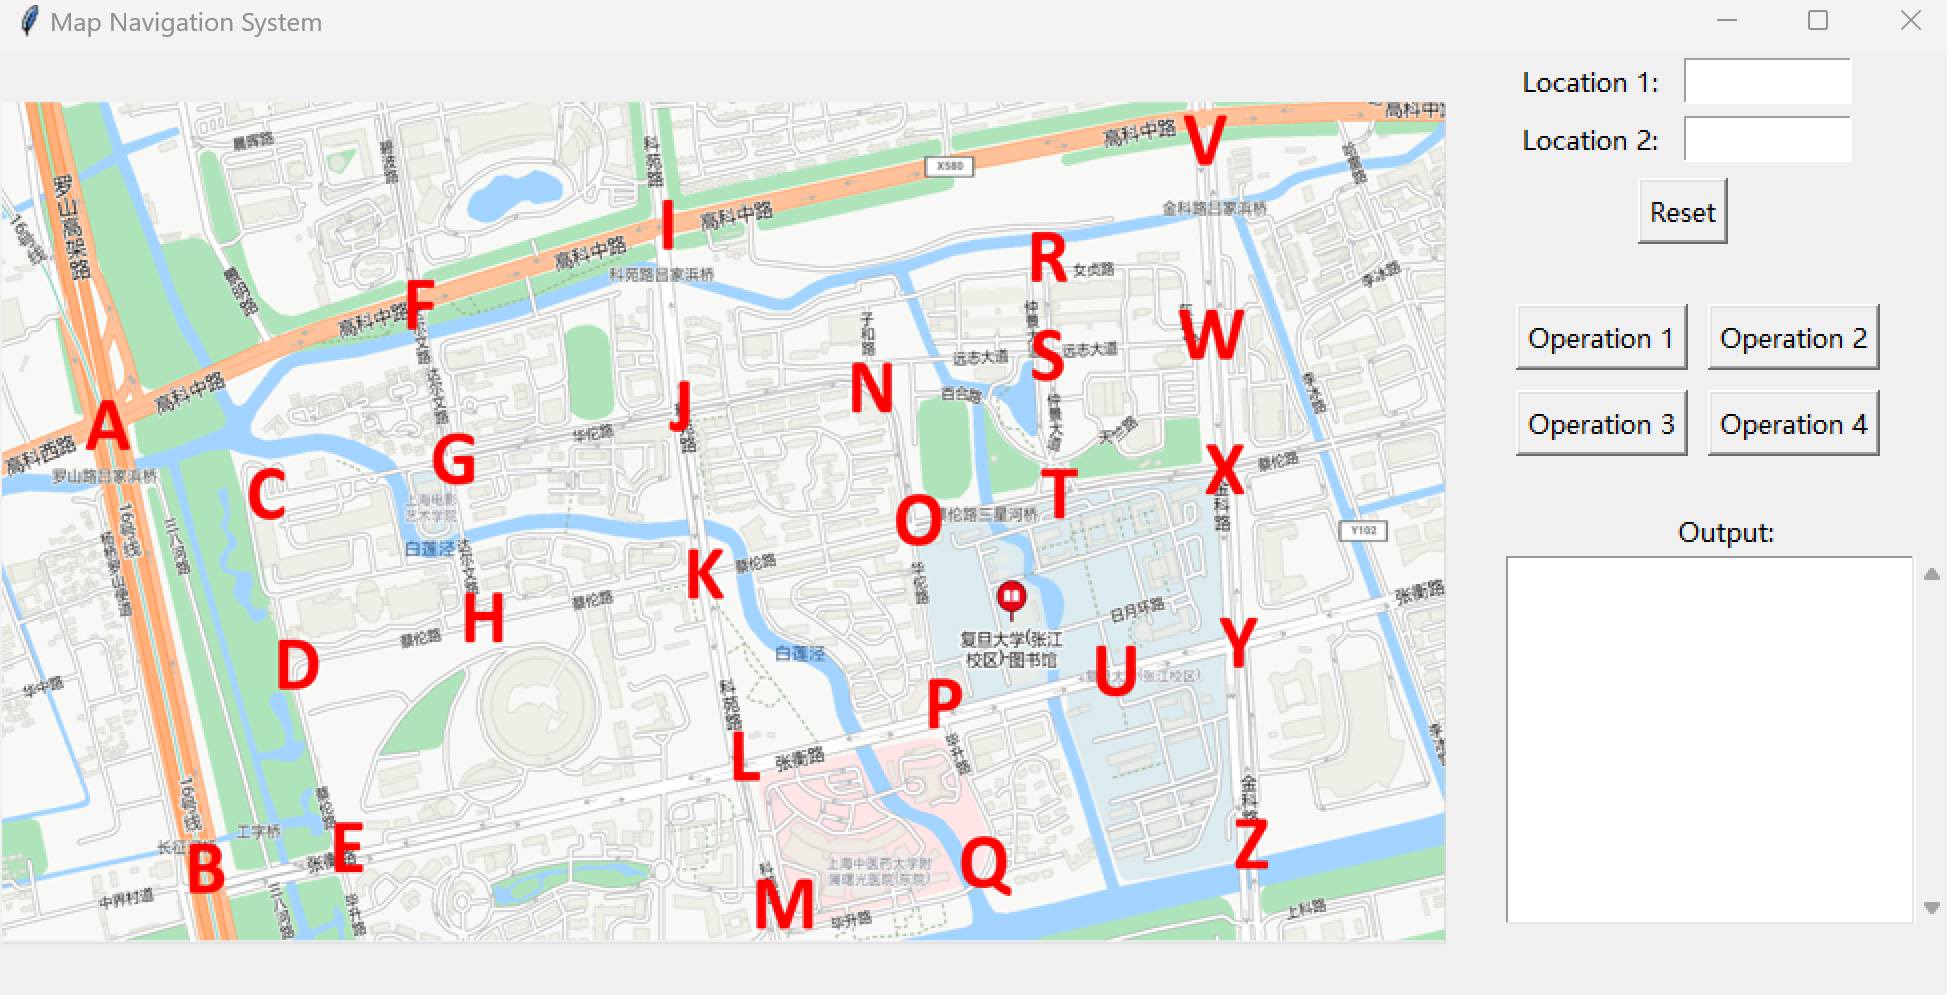
\includegraphics[width=0.8\textwidth]{gui.png}
    \caption{Interface of the map navigation system}
\end{figure}
The interface is divided into two parts, the left part is the map, and the right part is the operation area.\\
The map is part of Shanghai, and the key locations (vertices) are marked with capital letters.\\
The operation area is divided into three parts, the top part is the input area, the middle part is the operation buttons,
and the bottom part is the output window.\\
One can use the GUI as following instructions:\\
1. Type the capital letter of the key location in the input area, and click the button to perform the operation.\\
2. Or you can also click the center of the letters on the left picture, and the input area will automatically be written the location.\\
3. Click `Reset' to eliminate all the lines on the map, input and output.\\
4. Operation 1 is used to show all the shortest paths between two given locations, requiring two inputs.\\
5. Operation 2 is to display the shortest paths from all locations to a given location, requiring one input.\\
6. Operation 3 gives a subway route design, and the input is either none to call the Kruskal's algorithm or 1 root location to call the Prim's algorithm.\\
7. Operation 4 is to provide a bus route planning, and the input is the starting location.\\

\section{Results display}
Here are some results of the map navigation system.\\
\begin{figure}[htbp]
    \centering
    \begin{subfigure}{0.45\textwidth}
        \centering
    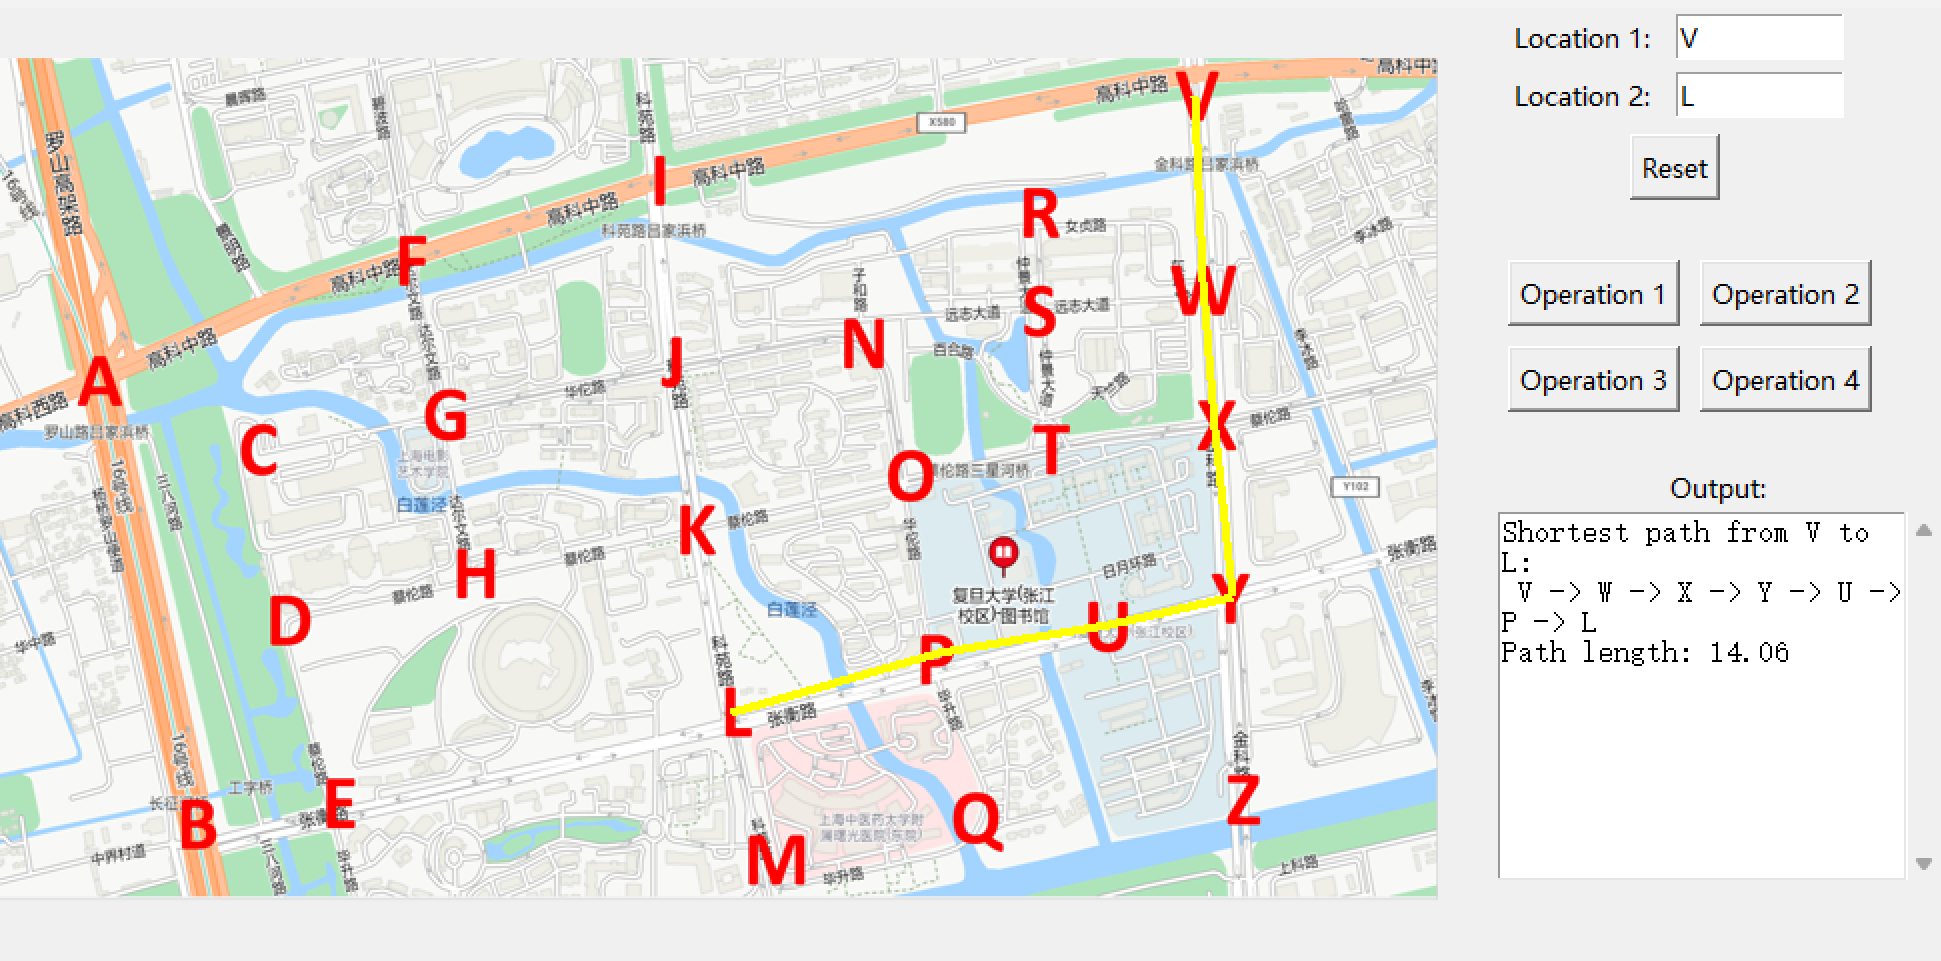
\includegraphics[width=\textwidth]{op1.png}
    \caption{Result of operation 1}
    \end{subfigure}%
    \hfill
    \begin{subfigure}{0.45\textwidth}
        \centering
    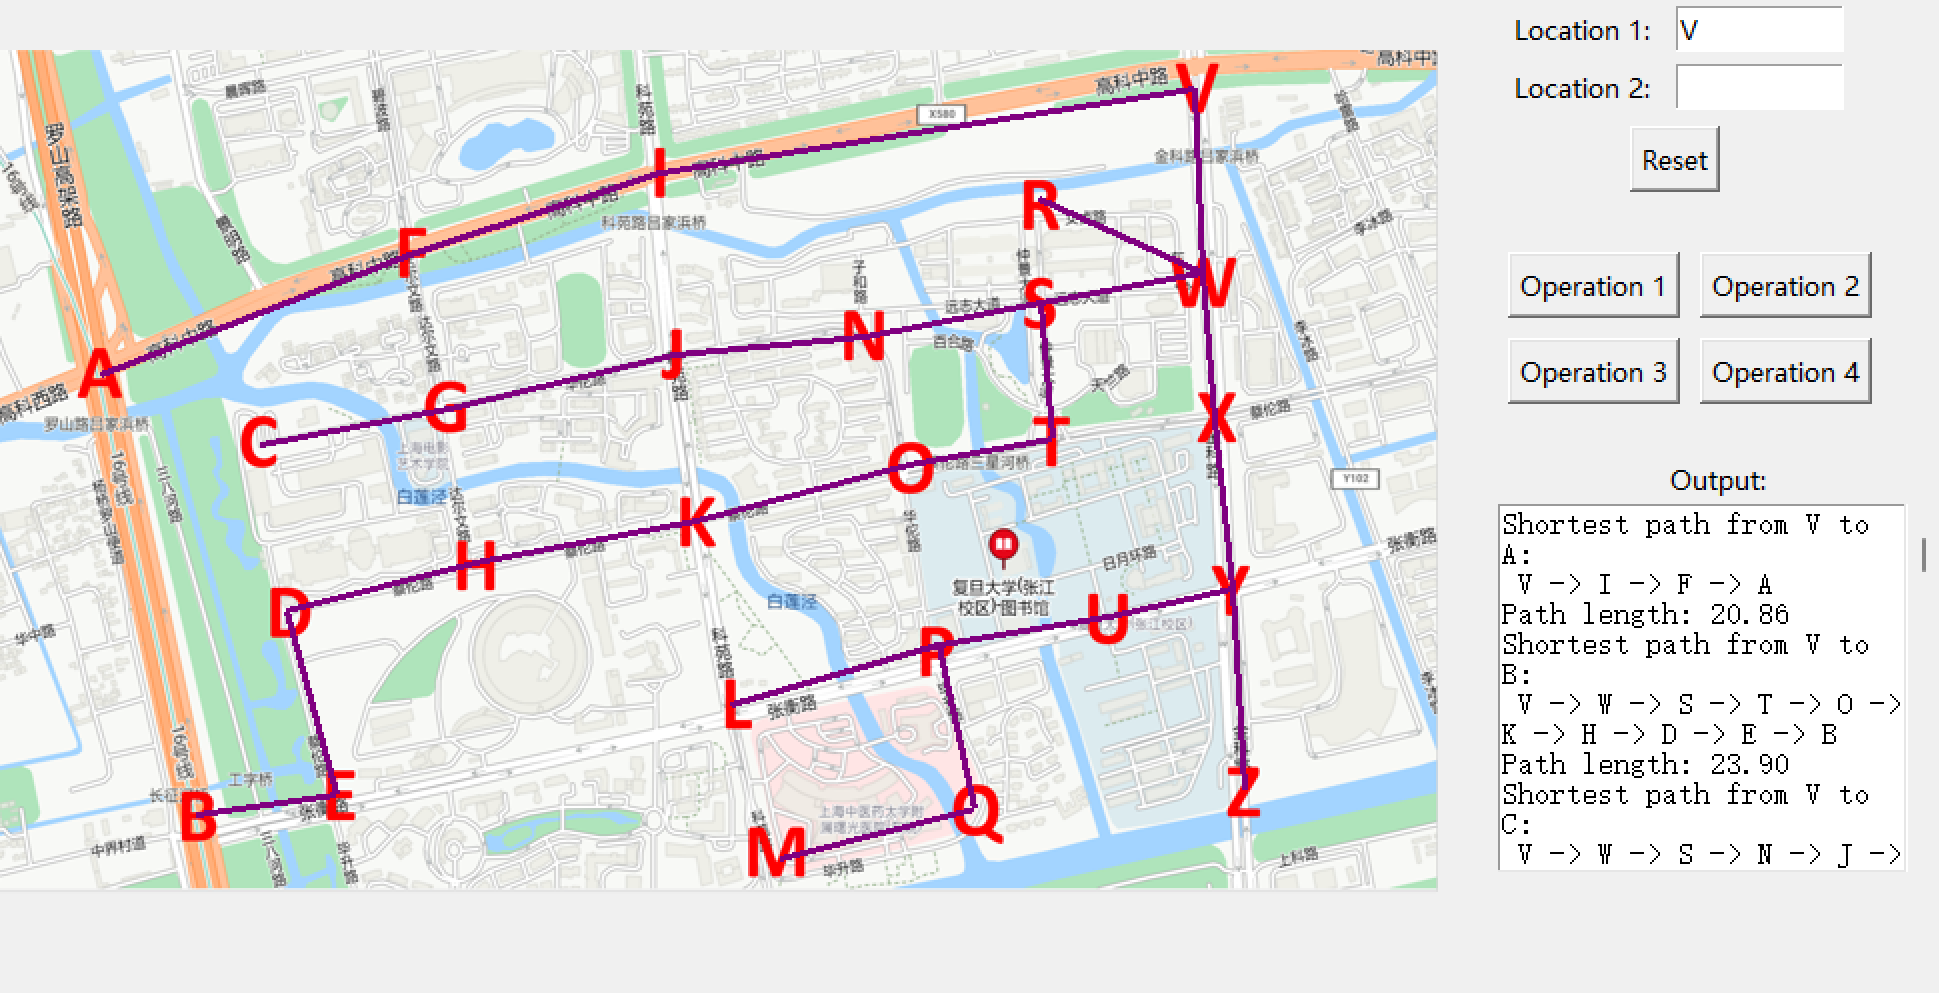
\includegraphics[width=\textwidth]{op2.png}
    \caption{Result of operation 2}
    \end{subfigure}%
    \vspace{0.5cm}
    \begin{subfigure}{0.45\textwidth}
        \centering
    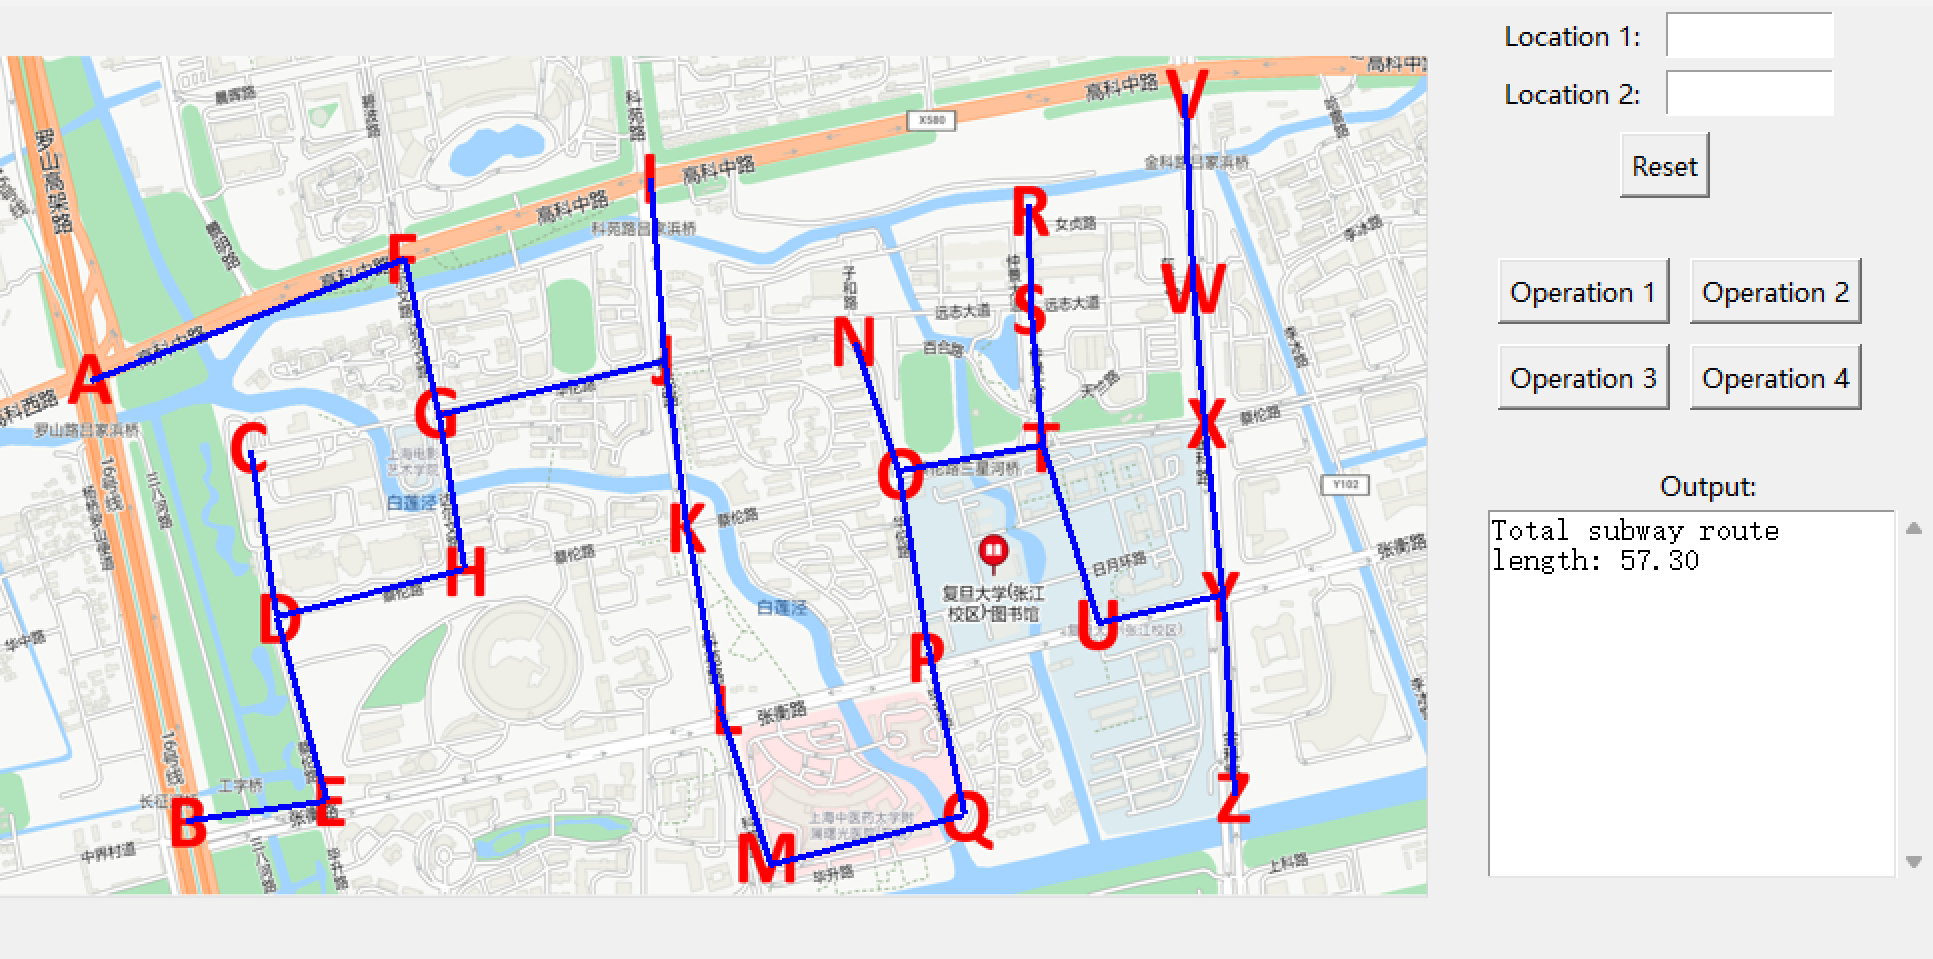
\includegraphics[width=\textwidth]{op3.png}
    \caption{Result of operation 3}
    \end{subfigure}
    \hfill
    \begin{subfigure}{0.45\textwidth}
        \centering
    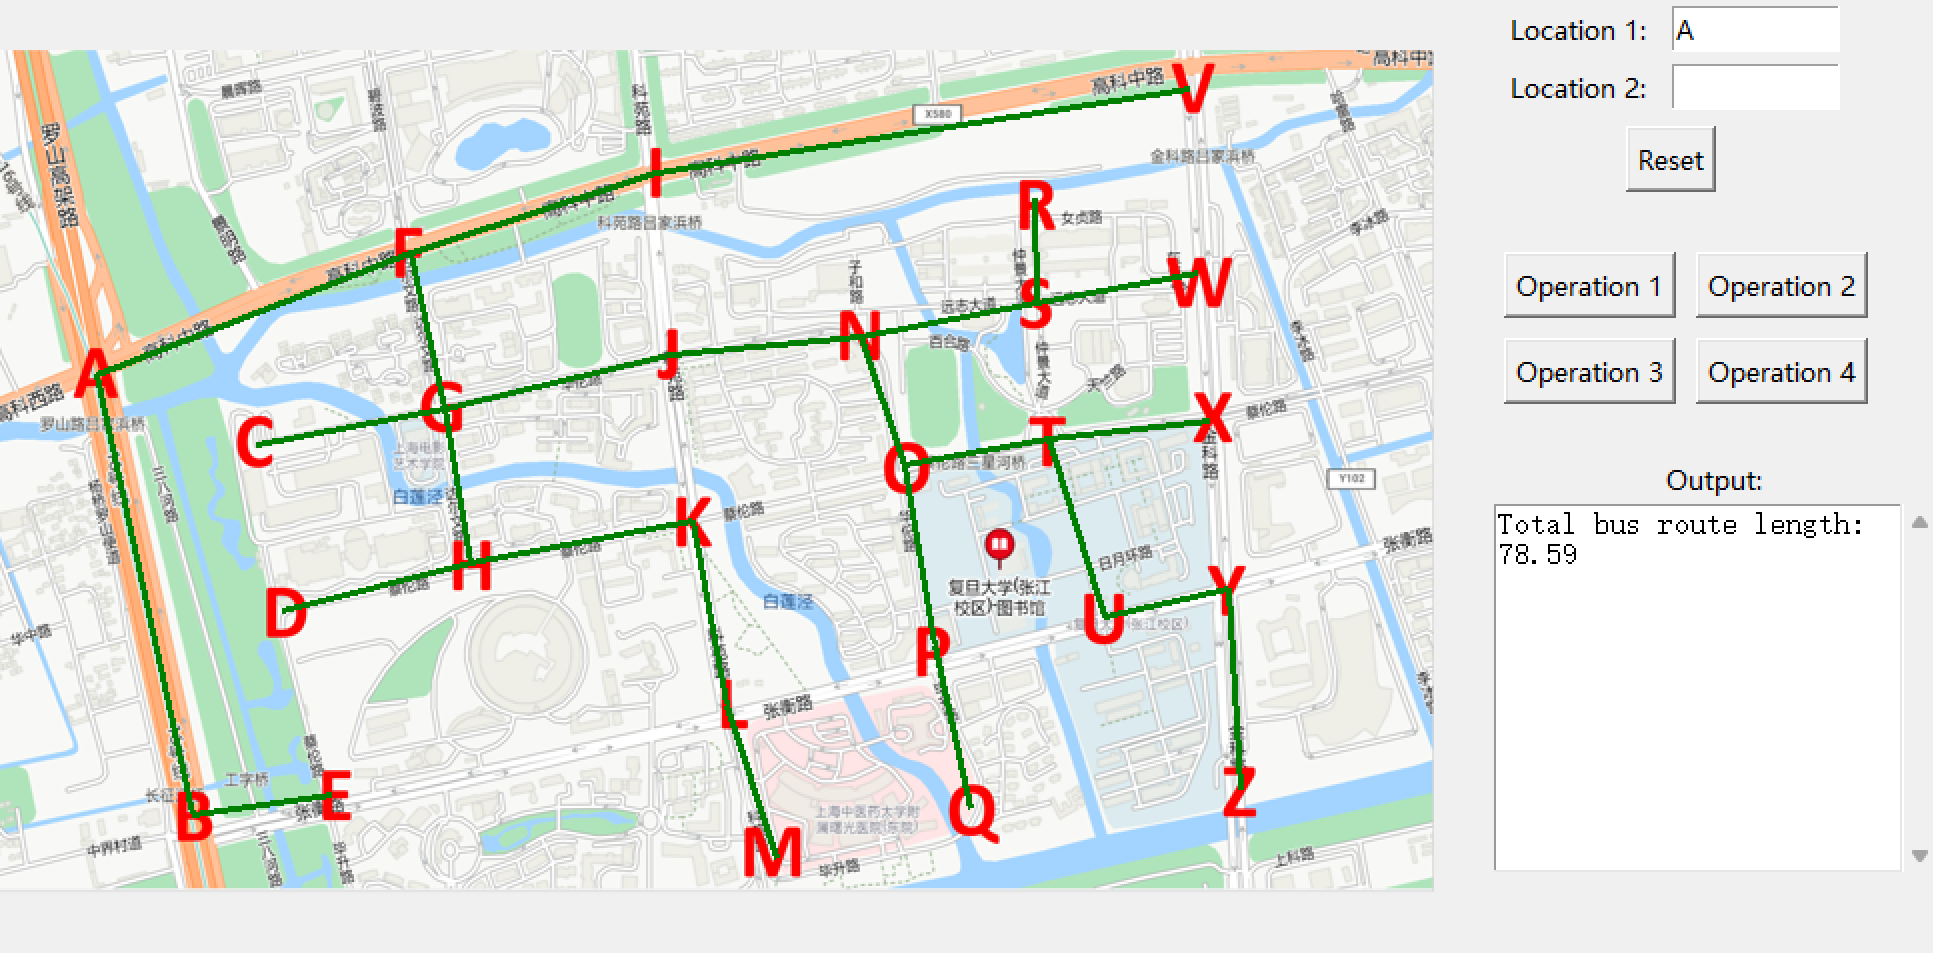
\includegraphics[width=\textwidth]{op4.png}
    \caption{Result of operation 4}
    \end{subfigure}%
    \caption{Results of the map navigation system}
\end{figure}


\section{Discussion}

\subsection{Bonus}
We have implemented the following bonus features:\\
1. \textbf{Multiple algorithms}\\
For the shortest path problems, we have implemented two algorithms, Dijkstra's algorithm and Floyd-Warshall algorithm.
For the MST problem, we have implemented Prim's algorithm and Kruskal's algorithm.
These solutions are based on different ideas, and can be used in suitable scenarios.\\
2. \textbf{Multiple solutions}\\
For the shortest path problems, we have implemented modified algorithms to record all the possible shortest paths between two vertices.
Since our case is unique of shortest paths, we test by changing all the weights to 1, and print all the solutions.
For brevity, we only draw the first path on the map.
\begin{figure}[H]
    \centering
    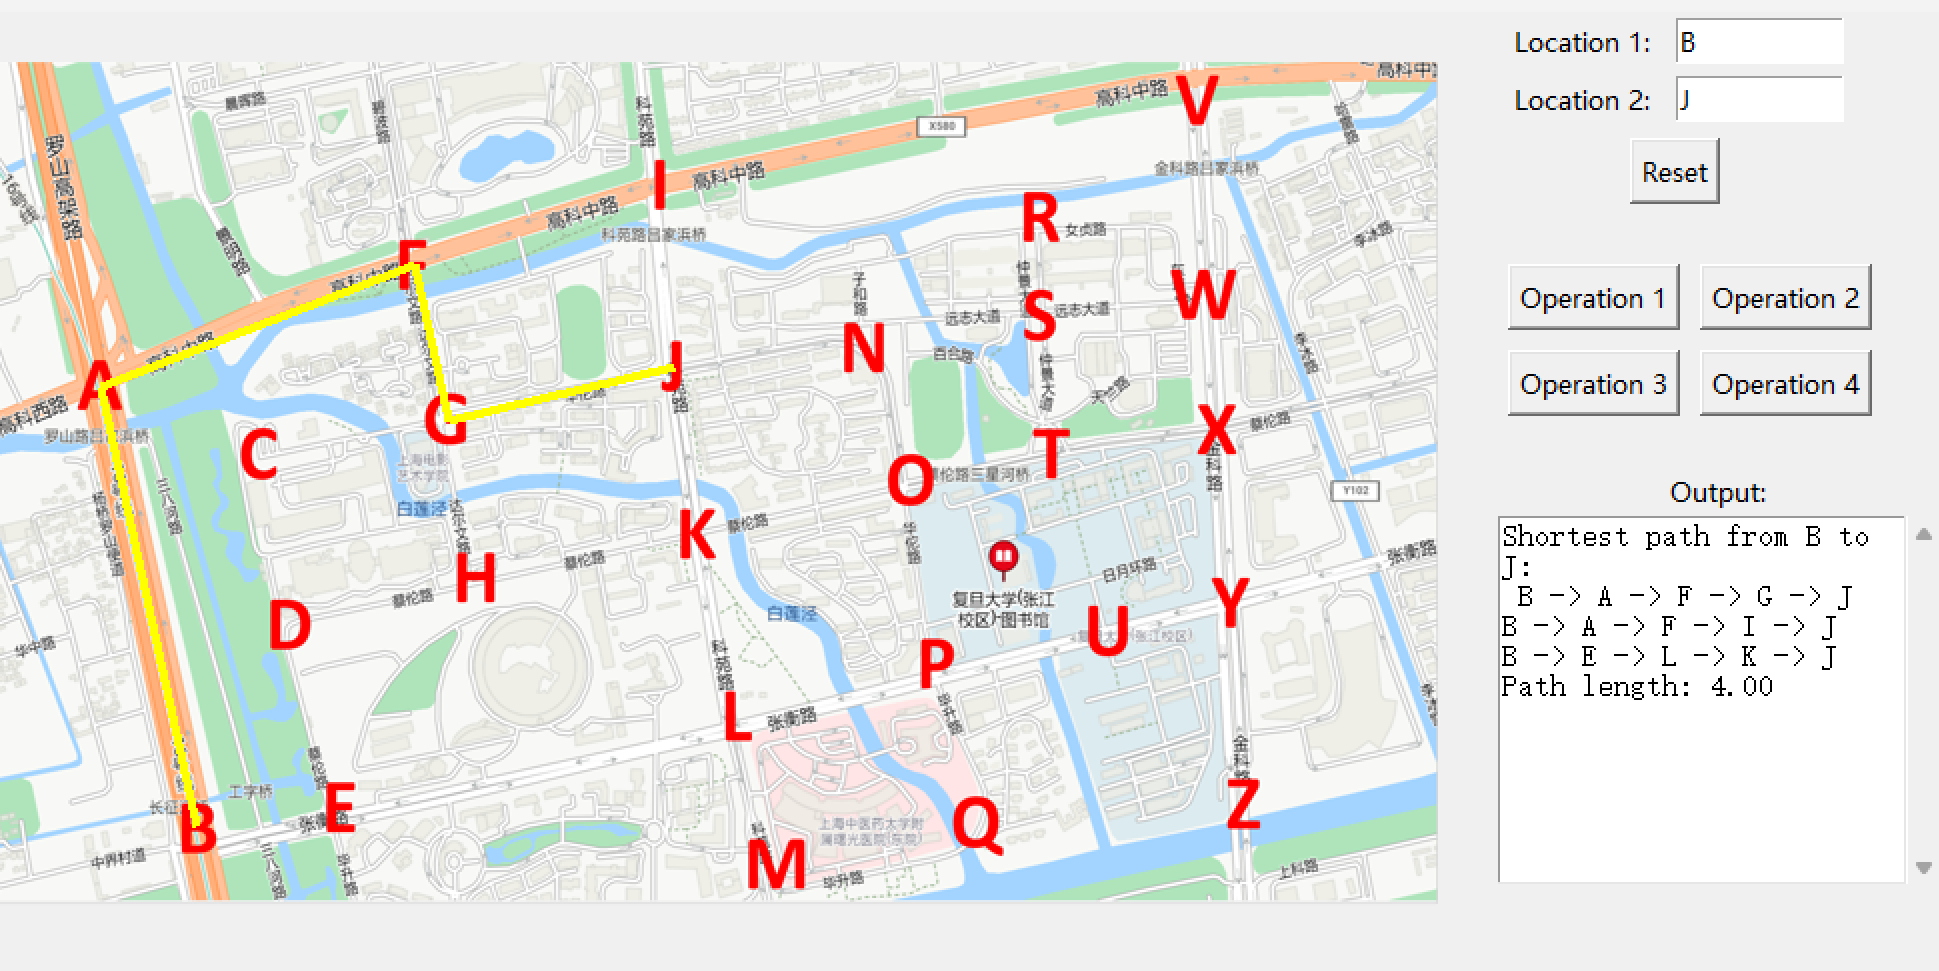
\includegraphics[width=0.7\textwidth]{all.png}
    \caption{Multiple solutions example}
\end{figure}
3. \textbf{Interactive GUI}\\
The GUI is supportive of clicking the map directly as an input, which provides comfortable usage.

\subsection{Limitations and future work}
The current implementation of the map navigation system has several limitations that could be addressed in future work:

\begin{enumerate}
    \item \textbf{Comprehensive MST Exploration:} Future efforts could focus on identifying all possible Minimum Spanning Trees (MSTs) using more advanced and specialized algorithms. This would offer a broader range of options for route optimization and network design.

    \item \textbf{Optimized Data Structures:} The current implementation's space complexity is relatively high, primarily due to the use of triple nested lists in the \textit{allpaths} data structure. Future work should explore more space-efficient data structures to manage and process graph data more effectively.

    \item \textbf{Enhanced Approach for Q4:} The current brute-force method in Q4 can be improved. Future research should investigate more sophisticated algorithms that can optimize the process, enhancing both performance and efficiency.

    \item \textbf{GUI Enhancements:} The existing GUI design, while functional, lacks aesthetic appeal and user-friendly features. Future iterations of the system should incorporate a more visually engaging design and a more intuitive layout, thereby improving user experience and interaction.
\end{enumerate}

These areas represent key opportunities for advancing the system's capabilities and usability.

\begin{thebibliography}{9}
\bibitem{CLRS}
Cormen, T. H., Leiserson, C. E., Rivest, R. L., Stein, C. (2022). 
\textit{Introduction to Algorithms} (4th ed.). The MIT Press.
\end{thebibliography}

\end{document}